\section{An interpreter for CRN++}

In the article \textit{CRN++: Molecular Programming Language}, Marko Vasic, David Soloveichik, and Sarfraz Khurshid define a language for programming chemical reactions to perform computation. They define a context-free grammar for this language and explain some of the limitations of the uses and expressiveness of the language when real-world chemical reactions enter the equation. 


\subsection{Grammar}

Looking at the grammar defined by the article in their listing 1.1, there are immediately some changes we would like to make. Besides this, we impose a few syntactic restrictions to ensure all parsed programs behave as expected. 

In the following, our changes to the grammar is listed. The complete revised grammar can be seen in appendix \ref{sec:grammar_revised}. 




As stated in the article, the rule \texttt{ConcS} represents the starting concentration of the species. Thus a \texttt{conc['$\langle \text{A} \rangle$', '$\langle \text{64} \rangle$']} on line 32, effects the the concentration of \texttt{A} on line 16. We deemed this non-intuitive, and to force the concentrations to be stated at the top of the program. This was done by changing the \texttt{RootList}:
\begin{tabbing}
    $\langle \text{Crn} \rangle$ \,::=\; \= \texttt{crn= \{'$\langle \text{ConcList} \rangle$' ',' $\langle \text{StepList} \rangle$}\} \\
    
    $\langle \text{ConcList} \rangle$ \,::=\;  $ \epsilon$ \\
    
     \>\textbar \, $\langle \text{Conc} \rangle$ ',' $\langle \text{ConcList} \rangle$ \\

      $\langle \text{StepList} \rangle$ \,::=\;  $\langle \text{Step} \rangle$ \\

      \>\textbar \, $\langle \text{Step} \rangle$ ',' $\langle \text{StepList} \rangle$ \\
\end{tabbing}
Furthermore, in \texttt{CommandS} \texttt{ArithmeticS} is mentioned but not defined. We assume that it refers to the defined but not mentioned \texttt{ModuleS}, which would make much sense now that \texttt{ModuleS} contains arithmetic expressions. Therefore, we rename \texttt{ArithmeticS} to \texttt{ModuleS}.\\

Other than \texttt{ConcS}, there are also other restrictions, all of which we found easier to implement using syntactic restrictions. Firstly, all \texttt{number} must be non-negative, since chemical concentrations are always positive. Furthermore, to ensure fast and deterministic convergence of all ODEs, there can not be any cycles where one species depends on itself nor can a species be written to twice in one step. This implicitly disallows multiple \texttt{cmp} now that all \texttt{cmp} write to the same flags. Lastly, we enforce that all \texttt{ConditionalS} in a step must be mutually exclusive, e.g. \texttt{ifLT} cannot be used together with \texttt{ifLE} since both can be true simultaneously and that there can not be any nested \texttt{if}. This does not reduce expressiveness and makes it simpler to check the restrictions.



\subsection{Abstract syntax tree (AST)}
The AST is rooted in Root: 
\begin{minted}{haskell}
    type Root = R of Conc List * Step List
\end{minted}
Which forces all the \texttt{Concs} to come before the steps, where Conc is defined as:
\begin{minted}{haskell}
    type Conc = C of species * float
\end{minted}
This is then followed by all the \texttt{Steps}:
\begin{minted}{haskell}
    type Step = S of Command List
\end{minted}
Where the definition of \texttt{Command} is:
\begin{minted}{haskell}
    type Command =
        | Ld of species * species
        | Add of species * species * species
        | Sub of species * species * species
        | Mul of species * species * species
        | Div of species * species * species
        | Sqrt of species * species
        | Cmp of species * species
        | Rx of species List * species List * float
        | IfGT of Command List
        | IfGE of Command List
        | IfEQ of Command List
        | IfLT of Command List
        | IfLE of Command List
\end{minted}
And \texttt{species} is just a string, that signifies the name of the species:
\begin{minted}{haskell}
    type species = string
\end{minted}
The tree representation of the ..... program can be seen below:
\subsection{Parser}


\subsection{Type checker}
After parsing, we have an AST, however, this AST might not follow all the rules extraneous to the grammar. By recursively matching on each \texttt{StepList} in the AST, we check all the constraints mentioned in the section on the grammar, for example, that the conditionals in a step do not overlap and that no species is written to twice. While traversing the \texttt{StepList}, a graph $G$ is built, whose nodes represent species and an edge from $a\to b$ signals that $a$ is input to $b$. By then trying to topologically sort $G$, we can quickly check if $G$ is a $DAG$ and thereby does not contain any cycles.

\subsection{State and interpreter}
The state is quite simply just a map from each species to its corresponding value:
\begin{minted}{haskell}
    type State = Map<species, float>
\end{minted}
Since each \texttt{State} only depends on the last \texttt{State} and the steps, one can make an infinite \texttt{State} sequence, by implementing a function that generates the next state based on the current state:
\begin{minted}{haskell}
    let doStep (S(cl): Step) (state: State) : State = doCommandList cl state
\end{minted}
and utilizing it in an unfold. The interoperate function then becomes:
\begin{minted}{haskell}
    let interpretProgram (R(concl, stepl)) =

        if not (isTyped (R(concl, stepl))) then
            failwith "Does not typecheck"
        else
            let initialState = getInitialState concl
    
            Seq.unfold
                (fun (state, i) ->
                    let nextState = doStep (List.item (i % List.length stepl) stepl) state
                    Some(nextState, (nextState, i + 1)))
                (initialState, 0)
\end{minted}

Where \texttt{getInitialState} just reads all the initial concentrations:
\begin{minted}{haskell}
    let getInitialState (concl: Conc List) : State =
        List.fold (fun state (C(s, c)) -> Map.add s c state) Map.empty concl
\end{minted}

\subsection{Testing}
We wanted to use property based testing, in the hope that it would be as applicable here as it was when drawing trees in the first project. However, there were some obstacles. It was not easy to get \texttt{FsCheck} to generate an AST that could have resulted from a valid parsed program. Furthermore, generating programs and then parsing them was also not doable, since the fraction of valid programs over invalid programs is vanishingly small. Thus we opted for a more traditional approach to testing, where we have programs that we know are correct and programs that we know are flawed, and we make tests on these. \texttt{FsCheck} then picks one of these programs and we check that mapping shuffle on each \texttt{StepList} does not change whether it type checks or the resulting sequence of states. Since one cannot compare infinite sequences directly, we only check whether the first 50 steps match.\\

To increase the coverage of the tests, the individual arithmetic operators were tested in isolation, where \texttt{FsCheck} picks for example the numbers to add. These were then compared to the result from the arithmetic operations in \texttt{F\#}.

\subsection{Visualization}
To visualize the sequence of states, we first output the sequence to a file, in a manner where we can easily read it into Python.

We then load this into Python and get a list of all the species, and a matrix where row $i$ corresponds to the concentration in step $i$. The $j$th index in all rows refers to the concentration of the $j$th species, therefore, by transposing the matrix, the $i$th row becomes the data points that are to be plotted for species $i$. By then having two copies of each value except the last value, and having the x-axis $0,0.99,1,1.99,2,2.99\dots$ instead of $0,1,2\dots$ we get the stair plot that clearly shows the step-wise process instead of a continuous progression between steps.

To make the plot a bit nicer and easier to read, the lines have different opaque colours and one can elect which species are plotted through command line arguments. An example is shown in the following figure:
\begin{figure}[H]
    \centering
    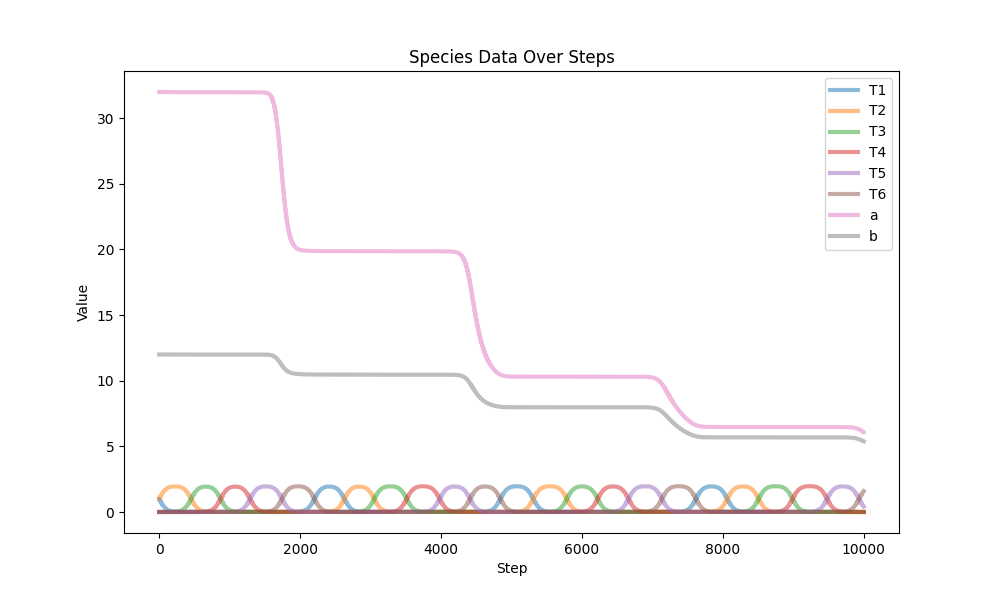
\includegraphics[scale=0.4]{report/figures/examplePlot.png}
    %\caption{Caption}
    %\label{fig:enter-label}
\end{figure}

\subsection{Assessment}